\documentclass[10pt]{article}
\usepackage{amsmath}
\usepackage{amssymb}
\usepackage{amsthm  }
\usepackage{fancyhdr}
\usepackage[margin=0.5in]{geometry}
\usepackage{graphicx}
\usepackage[utf8]{inputenc}
\usepackage{listings}
\usepackage{pdfpages}
\usepackage{standalone}
\usepackage{titling}
\usepackage{braket}
\usepackage{color}
\usepackage{hyperref}
\usepackage{wrapfig}
\usepackage{float}


\definecolor{dkgreen}{rgb}{0,0.6,0}
\definecolor{gray}{rgb}{0.5,0.5,0.5}
\definecolor{mauve}{rgb}{0.58,0,0.82}
\lstset{
  language=C,
  aboveskip=3mm,
  belowskip=3mm,
  showstringspaces=false,
  columns=flexible,
  basicstyle={\small\ttfamily},
  numbers=none,
  numberstyle=\tiny\color{gray},
  keywordstyle=\color{blue},
  commentstyle=\color{dkgreen},
  stringstyle=\color{mauve},
  breaklines=true,
  breakatwhitespace=true,
  tabsize=4
}

\newcommand{\NN}{\mathbb{N}} % Naturals
\newcommand{\ZZ}{\mathbb{Z}} % Integers
\newcommand{\QQ}{\mathbb{Q}} % Rationals
\newcommand{\RR}{\mathbb{R}} % Reals
\newcommand{\CC}{\mathbb{C}} % Imaginaries
\newcommand{\HH}{\mathbb{H}} % Quaternions
\newcommand{\FF}{\mathbb{F}} % Field

\newcommand{\ud}{\,\mathrm{d}} % Single-var differential (use like \partial)

\newcommand{\CoulombConstant}{\frac{1}{4\pi\epsilon_0}}

\DeclareMathOperator{\erf}{erf} % Error Function
\DeclareMathOperator{\erfc}{erfc} % Complementary Error Function
\DeclareMathOperator{\erfi}{erfi} % Imaginary Error Function
\DeclareMathOperator{\row}{row} % Matrix Row
\DeclareMathOperator{\col}{col} % Matrix Column
\DeclareMathOperator{\trace}{tr} % Matrix Trace
\DeclareMathOperator{\proj}{proj} % Vector Projection

\title{PHYS 319 Final Project: PWM-Based Synthesizer}
\author{Ashtan Mistal}
\date{April 2022}

\begin{document}

\maketitle

\break

\tableofcontents{}

\break

\section{Abstract}\label{sec:abstract}

% [abstract here]

\section{Introduction}\label{sec:introduction}

% [introduction here]
Exploration into the possibility of creating a user-controlled, MIDI\footnote{musical instrument digital interface}-compatible fully featured synthesizer has held a personal interest shortly after I became interested in music production itself.
Motivation for this project to encompass this personal interest stemmed from first using pulse width modulation to change the brightness of a bulb during an earlier lab.
Since my more recent interest in audio equipment itself, I was motivated to do an audio-related project.
The purpose of this project, as a result, was to help me gain a further understanding into the inner workings of oscillators and envelope generators, gain an appreciation for the MIDI standard, and of course to have a working, hand-made synthesizer for future music production related use.
All three areas of knowledge mentioned above would aid in future audio-related projects, both in software as well as in hardware, and help inspire for future related projects.
This project builds off of my previous related experience in music production, which provided me with a background on audio synthesis and processing.

\section{Theory}\label{sec:theory}
% A presentation of the theoretical background necessary to understand your project. Not every project will need a theory section, but most will. Here you would describe the physics of how sensors you use work (eg how does accelerometer measure acceleration, or how does a capacitive touch sensor work), or how an electrical interface to a device works.

In the following subsections, some basics regarding audio synthesis is discussed, as well as basics regarding the conversion methods needed for analog synthesizers. These basics provide a sufficient enough understanding behind the components necessary for both the 3 oscillator, MIDI compatible synthesizer, as well as the PWM-based synthesizer. 

\subsection{Digital - Analog Converter}\label{subsec:digital---analog-converter}

The primary goal of a digital to analog converter is to convert data bits (strictly HIGH or LOW), and convert to an analog signal with voltage varying on the values of the data bits.
This can be done either by receiving all data pins at once, or sending the data pins individually along with a clock bit, which is then read by a segment in the integrated circuit that decodes the data.
Receiving all data pins at once does not require the use of an integrated circuit, and can be done using resistor ladders \cite{TERRELL1996337}. 
More details regarding resistor ladders will be shown in Section~\ref{subsec:apparatus-details}.
Nonetheless, the DAC allows us to input a certain number of bits, in the case of this project, 10 bits, and convert to an analog signal (thereby giving us 1024 different values from 0 volts up until the maximum voltage).
This is essentially "receiving what output voltage to emit in binary", so that 1111111111, all pins on, corresponds to the maximum voltage, and 0000000000 (all pins off) correspond to minimum voltage, and something like 1101100110 till be $\frac{870}{1023}$ of the maximum. 

\subsection{Analog - Digital Converter}\label{subsec:analog---digital-converter}

An analog to digital works in the exact opposite way as a digital to analog converter.
By taking in an input voltage (as a proportion of the maximum voltage), an analog to digital converter will set some data value to be equal to that input voltage as a binary proportion to the maximum (or reference) voltage.
In the case of the microprocessor, this reference will be 3.3 volts.
The usage of this in the project is to be able to perform certain actions based on the value of this input pin, i.e. control the frequency based on what notes are being pressed. 

\subsection{Low Pass Filter}\label{subsec:low-pass-filter}

The theory behind an analog low pass filter is relatively simple;
the signal is sent through an RC circuit (see Figure~\ref{fig:LPF}), which, due to the charging and discharging properties of a capacitor, allows us to block frequencies past a certain cutoff frequency.
This cutoff frequency is given by the following formula:

\[
f_{cutoff}=\frac{1}{2 \pi R C},
\]

where $R$ is the resistance of the resistor in the circuit, and $C$ is the capacitance of the capacitor. 

So, in order to reduce unnecessary signal noise, we can apply a low pass filter to block frequencies past the human range of hearing, as well as attenuate higher pitched distortion coming from the circuit. 

In the specific case of this project, a 9.55 nF capacitor was made available.
Using the formula mentioned above, we can set the cutoff frequency to 20 kHz, therefore using a resistor of 800 Ohms. 

\begin{figure}[H]
    \centering
    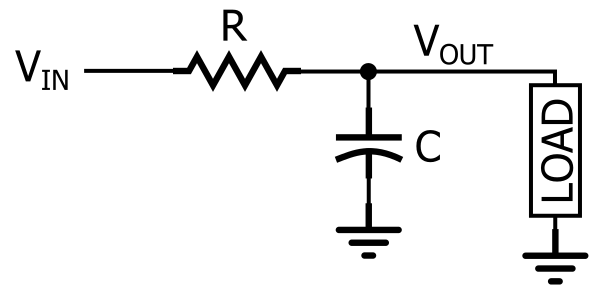
\includegraphics[width = 0.4 \textwidth]{lowpassfilter}
    \caption{A basic circuit diagram of a low pass filter \cite{keim_2019}. } % cite here
    % https://www.allaboutcircuits.com/technical-articles/low-pass-filter-tutorial-basics-passive-RC-filter/
    \label{fig:LPF}
\end{figure}

We can graph what the resultant signal graph will be post-LPF by using the following formula.
This formula is derived from the formula for a voltage divider circuit \cite{keim_2019}.



\[
V_{out}=V_{in}\left(\frac{X_{C}}{\sqrt{R_{1}^{2}+X_{C}^{2}}}\right), \quad X_{C}=\frac{1}{2 \pi f C}
\]

Hence, assuming $V_{in}$ is kept constant at 3.3 volts, we can view the output voltage as a function of the frequency, with $C = 9.55*10^{-9}$ F, and $R_1 = 800 \Omega$. 

\begin{figure}[H]
    \centering
    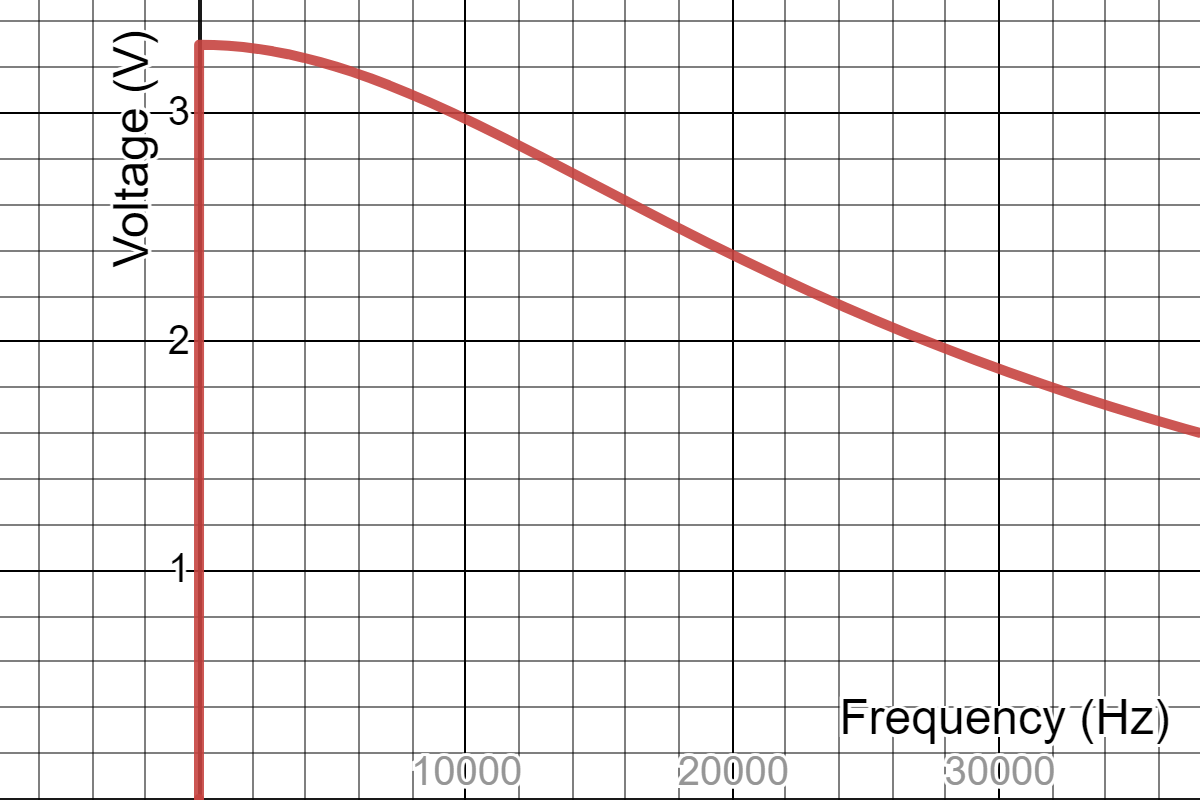
\includegraphics[width = 0.7 \textwidth]{lpfgraph}
    \caption{Plot of voltage versus frequency (linear scale) for an RC low pass filter. }
    \label{fig:lpfgraph}
\end{figure}

\subsection{MIDI Standard}\label{subsec:midi-standard-theory}
% https://www.instructables.com/Send-and-Receive-MIDI-with-Arduino/

Next, we delve further into details regarding the MIDI standard.
Note that this is strictly regarding the standard, and details regarding receiving MIDI data on the microprocessor will be described in Section~\ref{subsec:previous-apparatus-renditions}.

Sending MIDI data works by sending a stream of bytes at a given baud rate\footnote{The rate at which information is transferred in a communication channel.}. \cite{phongchit_2016} %https://www.setra.com/blog/what-is-baud-rate-and-what-cable-length-is-required-1#:~:text=The%20baud%20rate%20is%20the,of%209600%20bits%20per%20second.
This data is then decoded and processed, and instrument-related actions are taken accordingly. 

MIDI data is sent in either 2 or 3 bytes of information, depending on what the first byte is.
The first byte is always a command byte, as we see in Table \ref{tab:midi_command_bytes}. \cite{ghassaei_instructables_2017}
\begin{table}
    \centering
    \begin{tabular}{|c|l|}
    \hline
        10000001 & \text { note off } \\
        10010001 & \text { note on } \\
        10100001 & \text { aftertouch } \\
        10110001 & \text { continuous controller } \\
        11000001 & \text { patch change } \\
        11010001 & \text { channel pressure } \\
        11100001 & \text { pitch bend } \\
        11110001 & \text { non-musical commands } \\
        \hline
    \end{tabular}
    \caption{MIDI Command Bytes}
    \label{tab:midi_command_bytes}
\end{table}

\[
\begin{array}{l|l}

\end{array}
\]

The latter half-byte in the command is what channel the command is being sent on (in this case, they are all being sent on channel 1. 
With specific regards to this project, MIDI commands were just being sent through Channel 1 for simplicity's sake. 

If the command is a Note On, Note Off, or aftertouch, the first byte that is sent after the command is what note was pressed, and the second is the velocity value or aftertouch value, respectively. If the command is a controlled change or similar, the first byte that is sent after the command is what controller number was changed, and its new value. We are ignoring aftertouch, patch change, channel pressure, pitch bend, and non-musical commands in this project. 

Hence, we can read the first byte, quickly decode it, and read the second byte and third byte accordingly.
The C implementations are in Appendix~\ref{sec:appendix-b:-c-code-for-decoding-midi-data}.
When reading a note on / off command, the second byte corresponds to what note is being played.
There is a direct conversion from the MIDI note to the frequency, through the following formula:

% include formula to convert from midi to frequency
\[
f_{note}=440\times\frac{2^{(n-69)/12}}{1},
\]

where $n$ is the MIDI note number.
This frequency is then converted into the period of the note, and then converted into microseconds.
Because this formula is expensive to calculate, we used a lookup table to store the values of the frequencies.
This lookup table is in Appendix~\ref{sec:-table-of-notes-to-frequency-values}.

\subsection{PWM-Based Synthesis}\label{subsec:pwm-based-synthesis-theory}

PWM-based synthesis generates a square waveform from a given frequency, and a given amplitude.
The waveform generator is built into the microprocessor, and is controlled by the period and duty cycle of the waveform.

The theory behind this is relatively straightforward.
Below is a diagram of the PWM waveform.

\begin{figure}[H]
    \centering
    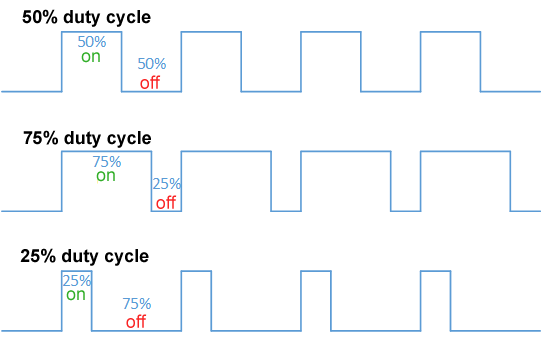
\includegraphics[width = 0.7 \textwidth]{pwmwaveform}
    \caption{PWM waveform \cite{pwm}} %\href{https://en.wikipedia.org/wiki/Pulse-width_modulation#/media/File:Duty_Cycle_Examples.png}}
    \label{fig:pwmwaveform}
\end{figure}

For this project, we used the PWM generator to generate a square waveform which was then outputted to an AUX output.

The PWM was used once it was determined that multi-oscillation was too computationally expensive (more discussed in Section~\ref{subsec:pwm-based-synthesis-apparatus}).


\subsection{ADSR Envelope Generation}\label{subsec:envelope-generation-theory}

Modern synthesizers do not just have a note ON / OFF transition when playing. An envelope is what allows one oscillator to be played like a pluck, to a pad, to  numerous other types of sounds. An ADSR envelope is controlled by 4 crucial parts:


\begin{enumerate}
    \item Attack phase. The attack phase controls how long it takes from the initial note press to when the amplitude is at its maximum. When the attack is short (like we'd want on a pluck), the maximum amplitude is reached very quickly, whereas when the attack is long (like we might want on a pad or string-type instrument), the maximum amplitude is reached much more slowly. 
    \item Decay Phase. Once the note reaches its maximum amplitude from the attack stage and the note is still on, the decay phase controls the time it takes for the note to decay from the attack phase to the sustain level (explained below). For a pluck-like instrument, we will want this decay time to be relatively short, for example, as this shapes the sound to only be heard for a short amount of time regardless of the time that the note is played for. 
    \item Sustain Phase. So long as the note is still on, this is the amplitude of the output (as a fraction of the input amplitude, so a note with a lower velocity will have a sustained amplitude of the same fraction, but not the same volume, as a note with a higher velocity). 
    \item Release Phase. As soon as the note is released (regardless of what phase it is in), the envelope will go into the Release phase, where the rate at which the output level decays from its initial volume before the release phase to its final level (0 volume, or -$\infty$ dB) is controlled. For a slow release, the release would be long (likely useful for pads or other slow-decaying instruments). 
\end{enumerate}

Due to debugging other issues, the envelope generation for this project did not work as anticipated (and was a low priority issue, compared to getting the waveform generators to work). Nonetheless, the code for the envelope generator in progress is shared in Appendix \ref{sec:appendix-c:-adsr-envelope-code}. 

\section{Apparatus}\label{sec:apparatus}
% Description of the project including diagrams of electrical and mechanical aspects. Depending on the complexity of the circuitry, a separate block diagram that shows functional blocks might be beneficial in addition to complete electrical schematics. The text should provide details on how the apparatus works. This section should also include a description of how your project is used.

\subsection{PWM Based Synthesis Apparatus}\label{subsec:pwm-based-synthesis-apparatus}

The actual PWM was generated on the MSP430G2553 microcontroller.
There was no need to send the signal to a DAC, as the PWM signal was directly sent to the AUX output.
This AUX output was then connected to a speaker.
The goal of having an AUX output was to be able to analyze the signal on a computer, instead of having to use a microphone to record the signal which would lead to a less accurate representation of the signal.
This also allowed for the synthesizer to be connected to a more powerful speaker.

The actual circuit diagram for the output is very simple, and will be included in Section~\ref{subsec:apparatus-details}.


\subsection{Apparatus Details}\label{subsec:apparatus-details}

The final rendition of this project is relatively simple in terms of electronics.
We begin by sending a signal of the same voltage to 10 different buttons, which act as the user control for the frequency of the wave emitted from the PWM\@.
These buttons then go into a 10-bit DAC, which was done using a resistor ladder based on the R-2R architecture, where the resultant signal is read through a 10-bit ADC (thus allowing for the same level of precision for the DAC as is available for the ADC) that is built into the MSP430G2553 microprocessor. % expand more

% include circuit diagram

\subsection{How the project is used}\label{subsec:how-the-project-is-used}

The project is intended to be used similarly to a piano, with the 10 buttons available corresponding to various keys on a piano, ranging from A4 to C6, excluding sharps and flats in the note range.
When these buttons are pressed, the corresponding amplitude of the input signal is changed.
This signal is decoded by the ADC, which changes the period of the PWM signal accordingly by modifying a global variable.
The duty cycle is then set to always be 50\%, by bit shifting the value of the global variable to the right by 1 bit.

\subsection{Previous Apparatus Renditions}\label{subsec:previous-apparatus-renditions}

As the initial intention of this project was to include MIDI compatibility, it is important to also include circuit diagrams for this, given it offered different methods of user interaction.
The rendition of the project that allowed for MIDI input was the 3 oscillator version (which, as will be discussed in the Results section, did not work properly due to hardware limitations).
Thus, the apparatus diagram below will reflect this


\section{Results}\label{sec:results}

% How did the device perform? Did it work according to the expectations? Comparison of theory to results obtained (as quantitative as possible). Problems encountered, graph(s) of data obtained, if appropriate, accuracy of the device (if it is a measuring instrument).
Unfortunately, the 3 oscillator version did not work properly due to software limitations.
When iterating through the different waveforms, the period set in the for loop was wildly inaccurate.
This was due to the fact that this was largely hardware-based, and did not use a timer to ensure accuracy of the period being set.
Hence, the actual period was based on the number of CPU cycles that were executed, which changed based on the period due to numerous factors.

Some of these factors include the use of multiplication, division, and modulo, which were not available in the MSP430G2553 microprocessor on a hardware level and thus were computationally expensive.
Because there was this large computational overhead, not only was the waveform itself inaccurate, but the MIDI data was unable to be processed in a timely manner.
The 3 oscillator version was therefore only able to act as a noise generator, and was not able to be used as a semi-realistic synthesizer.

Nonetheless, the PWM based, single oscillator version was much more accurate than the 3 oscillator version.
The PWM based version was able to accurately reproduce a square wave with a given period, mainly due to the fact that the PWM is based on a timer, which is able to accurately set the period and is also not based on the number of CPU cycles.


% TODO: 
% - Measure input on a FFT on Studio One (a spectral filter may be more accurate)
% - Compare to proper square wave
% - accuracy of the square wave frequency using a tuner



\section{Discussion}\label{sec:discussion}

% Discuss what went well, and what could have been better, possible improvements to the device.

It would have been a much better idea to use 3 PWM signals instead of 3 iterative waveforms, and modify the period and duty cycle accordingly to match the given waveform being played.
This would have allowed for a much more accurate representation of the waveform being played, and would have allowed for the use of a timer to accurately set the duty cycle.
Of course, this may have had its own limitations as well, as we would have to be accurately changing the duty cycle of the PWM signal, and this would have required another timer to be used, along with numerous interrupts.
This may have been a better idea, but still is at risk of being too computationally expensive due to the constant changing of the duty cycle with a semi-unknown period (due to the fact that we have so many notes that could be played)
Early analog synthesizers combated this problem, and simultaneously allowed for polyphony, by using a separate waveform generator for each note.
But alas, this is too expensive for our microprocessor, and the 3 oscillator version was not able to be used as a real-time synthesizer, and the PWM based version was not "interesting" enough for real-world use (albeit was much more accurate and actually playable).

The primary source of inaccuracy for the PWM based version was the DAC being used to convert the notes being pressed to an analog signal.
Precision resistors were not used, and so a lot of fluctiation was observed in the analog input signal.
This is observed in the FFT signal discussed inFigure~\ref{fig:fft}.

\section{Conclusions}\label{sec:conclusions}

% Was it worth constructing? What did you learn?



%include references here
% Sources other than the course lab manual or lab web page should be referenced. Especially if your code is based on code you found on the web or elsewhere, you should make sure that the body of your report contains a clear citation to the source you used, and a corresponding reference here in the references section. In the body of the report, you should also explain clearly what differentiates your code from the source you used.

\appendix

\section{Appendix A: Table of Notes to Frequency Values}\label{sec:-table-of-notes-to-frequency-values}



% Any additional material that should be included in the report, but not necessary for the main body can be included as appendices. You should definitely include (well-annotated) program listings.

\begin{table}[h]
    \centering
    \begin{tabular}{c|c}
         &  \\
         & 
    \end{tabular}
    \caption{Table of Notes to Frequency Values}
    \label{tab:pianonotestofrequency}
\end{table}

\section{Appendix B: C Code for Decoding MIDI Data}\label{sec:appendix-b:-c-code-for-decoding-midi-data}
Please note that functions regarding the actual waveform generation were ignored here for space and organization purposes. 

\begin{lstlisting}[label={lst:lstlisting}]
//
// Created by Ashtan Mistal on 2022-03-24.
//

#include "msp430.h"
#include "msp430g2553.h"

unsigned long frequency;
unsigned long amplitude;
unsigned long noteon;
unsigned long square_wave_volume;
unsigned long noise_wave_volume;
unsigned long triangle_wave_volume;
unsigned long sawtooth_wave_volume;
unsigned long attack_rate;
unsigned long decay_rate;
unsigned long sustain_level;
unsigned long release_rate;

void send_output(int input) {
    P1OUT = input;
}

// take in MIDI note and convert to frequency
// midi note is a number between 0 and 127
int midi_to_frequency(int midi_note) {
    // this is a slow function because it declares a variable every time it is called
    // will be better to declare a global variable and use that instead
    int midi_to_frequency_table[128] = {
        8, 8, 9, 9, 10, 10, 11, 12, 12, 13, 14, 15, 16, 17, 18, 19, 20, 21, 23, 24, 25, 27, 29, 30, 32, 34, 36, 38, 41, 43, 46, 48, 51, 55, 58, 61, 65, 69, 73, 77, 82, 87, 92, 97, 103, 110, 116, 123, 130, 138, 146, 155, 164, 174, 184, 195, 207, 220, 233, 246, 261, 277, 293, 311, 329, 349, 369, 391, 415, 440, 466, 493, 523, 554, 587, 622, 659, 698, 739, 783, 830, 880, 932, 987, 1046, 1108, 1174, 1244, 1318, 1396, 1479, 1567, 1661, 1760, 1864, 1975, 2093, 2217, 2349, 2489, 2637, 2793, 2959, 3135, 3322, 3520, 3729, 3951, 4186, 4434, 4698, 4978, 5274, 5587, 5919, 6271, 6644, 7040, 7458, 7902, 8372, 8869, 9397, 9956, 10548, 11175, 11840, 12544};
    return midi_to_frequency_table[midi_note];
}


// midi data is sent in as serial peripheral data on ports P2.0 and P2.1
// convert the serial port input to an 8-bit integer
// this is the MIDI data
int serial_to_midi() {
    int i;
    int midi_data = 0;
    for (i = 0; i < 8; i++) {
        midi_data |= (P2IN & 0x01) << i; // assuming P2.1 is a 1 or 0; may have to change to be based on data and not clock
        // may have to delay cycles here based on baud rate -- or may have to remove for loop if baud rate cannot be changed and number of cycles is too high
    }
    return midi_data;
}


// decode the midi data to determine if it is a note on or a continuous controller change
// return if it is a note on or a continuous controller change
// if it is a note on, return 1
// if it is a continuous controller change, return 2
// else return -1
int decode_midi_data(int midi_data) {
    if ((midi_data & 0xF0) == 0x90) {
        return 1;
    } else if ((midi_data & 0xF0) == 0xB0) {
        return 2;
    } else if ((midi_data & 0xF0) == 0x80) { // note off
        return 3;
    } else {
        return -1;
    }
}

void handle_note_on(int midi_note, int velocity) {
    frequency = midi_to_frequency(midi_note);
    amplitude = velocity;
}

void handle_note_off() {
    noteon = 0;
    amplitude = 0; // set amplitude to 0 to turn off the note; remove this if we are using ADSR
    // amplitude will be handled by the release phase UNLESS we are removing the ADSR envelope

}

void handle_continuous_controller_change(int controller_number, int controller_value) {

    switch(controller_number) {
        case 1:
            square_wave_volume = controller_value; 
            break;
        case 2:
            noise_wave_volume = controller_value; 
            break;
        case 3:
            triangle_wave_volume = controller_value; 
            break;
        case 4:
            sawtooth_wave_volume = controller_value; 
            break;
        case 5:
            attack_rate = controller_value;
            break;
        case 6:
            decay_rate = controller_value;
            break;
        case 7:
            sustain_level = controller_value;
            break;
        case 8:
            release_rate = controller_value;
            break;
        default:
            break;
    }
}


/*
 * Steps to decode MIDI data:
 * 1. Read the first byte
 * 2. If the first byte is a note on, read the second and third byte
 * 3. If the first byte is a continuous controller change, read the second and third byte
 * 4. If the first byte is neither, return -1 and ignore the rest of the bytes
 */

// this is the interrupt service routine
void decoder() {
    int midi_data = serial_to_midi();
    int midi_data_type = decode_midi_data(midi_data);
    if (midi_data_type == 1) {
        int midi_note = serial_to_midi();
        int velocity = serial_to_midi();
        handle_note_on(midi_note, velocity);
    } else if (midi_data_type == 2) {
        int controller_number = serial_to_midi();
        int controller_value = serial_to_midi();
        handle_continuous_controller_change(controller_number, controller_value);
    } else if (midi_data_type == 3) {
        int midi_note = serial_to_midi();
        int velocity = serial_to_midi();
        handle_note_off();
    }
}




// enable an interrupt service routine based on the midi clock pin
void enable_interrupt() {
    P2IE |= 0x02; // enable interrupt on P2.1
    P2IES |= 0x02; // set interrupt to trigger on falling edge
    P2IFG &= ~0x02; // clear interrupt flag
    P2IE |= 0x02; // enable interrupt on P2.1
    _BIS_SR(GIE); // enable global interrupts
}

void __attribute__((interrupt(PORT2_VECTOR))) PORT2_ISR(void) {
    decoder();
    P2IFG &= ~0x01; // clear interrupt flag
}

int main(void) {
    P1DIR = 0b11111111; // set all pins on P1 to output
    P1OUT &= 0b00000000; // set all pins on P1 to 0
    // set up P2 input pins
    P2DIR = 0b00000000; // set all pins on P2 to input
    P2REN |= 0b11111110; // enable pull-up resistors on all pins on P2 except P2.0

    //// NOTE TO SELF that there is not in fact a clock pin on the MIDI cable.

    // initialize variables to some default values
    frequency = 2;
    amplitude = 255;
    noteon = 1; // can change to 0 if we do not want our synthesizer to be making noise when we turn it on
    square_wave_volume = 255;
    noise_wave_volume = 0;
    triangle_wave_volume = 255;
    sawtooth_wave_volume = 255;
    attack_rate = 2;
    decay_rate = 40;
    sustain_level = 127;
    release_rate = 127;



    // set up P2 interrupt
    enable_interrupt();
    unsigned long period = 1;

    while (1) {
        period = 1000000 / frequency; // period converted to microseconds
        unsigned long i;
        for (i = 0; i < period; i++) {
            int output = square_wave_volume * square_wave_iteration(period, i); // this is good
            output += noise_wave_volume * noise_wave_iteration(period, i)/4096; // this is good
            output += triangle_wave_volume * triangle_wave_iteration(period, i)/period; // this is good
            output += sawtooth_wave_volume * sawtooth_wave_iteration(period, i)/period; // this is good
            output = output / 4;
            output = output * amplitude / 128;
            output = ADSR(output, timestep_counter);
//            serial_output(output);
            send_output(output);
        }
}
\end{lstlisting}

\end{document}
